% Compile from docs/ric: pdflatex ric && bibtex ric && pdflatex ric && pdflatex ric
%
% Every table under tables/ and both figures are generated by
% experiments/ric_clover/make_report_assets.py from the result files in
% experiments/ric_clover/results/. Rerun that script after any new run; do not edit
% the generated tables by hand. Numbers quoted in the text that are not in a table
% come from the diagnostics listed in Section~\ref{sec:repro}.
\documentclass[11pt]{article}

\usepackage[margin=1in]{geometry}
\usepackage{amsmath,amssymb}
\usepackage{booktabs}
\usepackage{graphicx}
\usepackage{natbib}
\usepackage{hyperref}
\usepackage{xcolor}

\newcommand{\todo}[1]{\textcolor{red}{[#1]}}
\newcommand{\Nb}{N_{b}}
\newcommand{\Na}{N_{a}}
\newcommand{\Smat}{\mathbf{S}}
\newcommand{\Fmat}{\mathbf{F}}
\newcommand{\Real}{\mathbb{R}}
\newcommand{\Rhat}{\widehat{\mathbf{R}}}

\title{Spurious Dependence in a Coherent Hierarchical Forecaster:\\
Why CLOVER Fails on Cointegrated Series, and a Window-Realized Fix}

\author{\todo{author list}}
\date{\today}

\begin{document}
\maketitle

\begin{abstract}
CLOVER \citep{olivares2024clover} forecasts hierarchical time series coherently by
sampling a Gaussian factor model at the bottom level and aggregating every draw
through the summation matrix. Its authors report that it trails statistical
baselines on Australian Labour, a small, highly cointegrated hierarchy, and name
robustness to cointegration as future work. We locate the failure. It is not in
the predictive mean, which earlier error-correction variants targeted without
effect, but in the cross-series dependence. On Labour the Total's predictive
spread is $1.6$--$3.0$ times its forecast error, while the bottom level is
under-dispersed. CLOVER predicts a correlation of $+0.2$ to $+0.5$ between every
pair of bottom series. The realized innovations are correlated at about $-0.45$
between full-time and part-time siblings, a compositional relation that holds their
sum steady, and at about $+0.1$ elsewhere. The factor head reads each series' own
z-scored level history, and co-trending levels make every series look alike, so the
loadings align: the spurious-regression effect of \citet{granger1974spurious},
reproduced inside a neural head. We propose \emph{realized innovation correlation}
(RIC). It keeps the network's marginal variances and replaces its dependence with
the correlation of the window's first differences, shrunk toward a hierarchy-derived
target with an analytic intensity, then re-expressed as an exact factor model so
sampling, coherence and the training objective are unchanged. Over 12 paired seeds
with Holm correction, RIC improves scaled CRPS significantly on Prison ($-8.6\%$,
12/12 seeds) and on a synthetic hierarchy with known dependence ($-4.8\%$, 11/12). On
the synthetic data it recovers the true sibling correlation exactly ($-0.67$), where
CLOVER predicts the wrong sign. On Labour, CLOVER run with the paper's static and
calendar features still predicts the wrong sign. There RIC corrects the dependence,
narrows the over-dispersed aggregates and improves the paper's test window by
$2.5\%$ (11/12 seeds), but its overall gain under rolling origins is not significant.
Computing the same correlation from levels instead of differences gives no gain, which
isolates spurious level correlation as the cause. Scoring the joint bottom-level
distribution directly, with the energy and variogram scores, confirms the gains on
Prison and the synthetic hierarchy. It also exposes a cost that sCRPS hides: on
Traffic, a daily, seasonal hierarchy where CLOVER's learned dependence is already
good, RIC makes the joint distribution significantly worse ($+6$ to $+10\%$). A
pre-test backtest that selects on the energy score keeps RIC exactly where it helps
and rejects it on Traffic. Behind that gate, no dataset is significantly worse on any
score.
\end{abstract}

\section{Introduction}

CLOVER emits, for every bottom series $i$ and horizon $\eta$, a location
$\mu_{i\eta}$, an idiosyncratic scale $\sigma_{i\eta}$ and $K$ factor loadings
$\Fmat_{i\eta}\in\Real^K$, draws
$\hat b_{\eta} = \mu_\eta + \sigma_\eta\odot z + \Fmat_\eta\varepsilon$ with
$z\sim N(0,I_{\Nb})$ and $\varepsilon\sim N(0,I_K)$, clips at zero and aggregates
every draw through $\Smat$. Coherence holds by construction and the CRPS is
optimised on the aggregated samples \citep{olivares2024clover}. The implied
bottom-level covariance is $\operatorname{diag}(\sigma^2_\eta)+\Fmat_\eta\Fmat_\eta^\top$,
so the factor loadings alone decide how uncertainty adds up through the hierarchy.

The original paper reports that every deep model, CLOVER included, trails
statistical reconciliation on Labour. It attributes this to limited data, to
``strong trends and cycles, which can lead to artificially high correlations
between the series, resulting in spurious relationships'', and to cointegration,
naming robustness to it as future work. Earlier work in this project followed the
cointegration reading through the mean: Johansen \citep{johansen1991estimation} and
share-based cointegrating vectors fed to the encoder, a vector error-correction skip
on the location \citep{engle1987cointegration}, and loadings constrained to the
common-trend space \citep{stock1988testing}. None moved Labour by more than $0.0002$
sCRPS. This report explains why and gives a variant that does.

\paragraph{Contributions.}
\begin{enumerate}
  \item A diagnosis (Section~\ref{sec:diagnosis}). CLOVER's Labour gap is a dependence
  failure. The factor head produces near-parallel loadings from co-trending z-scored
  levels, so it predicts positive correlation everywhere. The real innovations carry
  negative within-parent correlation and a common component that fades over time.
  \item A method (Section~\ref{sec:method}). RIC re-estimates dependence in every window
  from first differences, shrinks it toward a target derived from $\Smat$ alone, and
  keeps the network's marginals and CLOVER's sampling, coherence and loss unchanged.
  \item Evidence (Sections~\ref{sec:results}--\ref{sec:ablations}): 12-seed paired tests
  with Holm correction across five public hierarchies, a synthetic hierarchy with known
  dependence, and ablations that isolate the cause.
  \item A corrected Labour baseline. The repository's Labour configuration lacked the
  paper's static and calendar features; restoring them closes most of the gap to the
  published CLOVER score.
\end{enumerate}

\section{Diagnosis: where CLOVER loses on Labour}
\label{sec:diagnosis}

Labour has 57 series (Total, 8 states, 16 state--gender nodes, 32 bottom series split
by full-time/part-time status), monthly, horizon 12. Its CLOVER configuration has no
cross-series mixer (hidden size 0 in the paper's Table~4), so each bottom series'
parameters are a function of its own z-scored 36-month window and its static
features only. The configuration in this repository also omitted the static and
calendar features that the paper's Table~4 lists. Adding them (status, gender and
state one-hots; month dummies) lowers CLOVER's Labour sCRPS from $0.0081$ to $0.0077$,
against $0.0074$ reported, which accounts for most of the gap between our baseline
and the paper's. We therefore treat the configuration with features as the Labour
baseline and report the featureless one alongside it. The diagnosis below holds
under both. Figure~\ref{fig:correlation} uses the featureless model. With features,
CLOVER predicts $+0.18$ ($h=1$) to $+0.30$ ($h=12$) for siblings, still the wrong
sign.

\paragraph{The mean is not the problem.} Replacing every predictive mean by the truth
(an oracle) lowers the Total's sCRPS only from $0.0044$ to $0.0038$ (seed~0). Most of
the Total's loss is therefore spread, not location.

\paragraph{Aggregates are over-dispersed, the bottom under-dispersed.} On the test
period the Total's predictive standard deviation is $2.0$--$2.8$ times its RMSE
without features ($1.6$--$3.0$ with them, Table~\ref{tab:levels}), and its 80\%
interval covers $97$--$99\%$ of outcomes. The bottom level's 80\% interval covers only
$66$--$73\%$ (Figure~\ref{fig:calibration}). With
a factor model, the only way to be too wide at the top and too narrow at the bottom is
to predict too much positive correlation between bottom series.

\paragraph{Predicted versus realized dependence.} Figure~\ref{fig:correlation} groups
bottom pairs by the depth of their lowest common ancestor in $\Smat$. CLOVER predicts
$+0.21$ to $+0.27$ for every class at $h=1$, rising to about $+0.4$ at $h=12$ (the
common-factor share of predictive variance grows from $0.50$ to $0.70$). The realized
innovations disagree in sign for siblings ($-0.45$): employment shifts between
full-time and part-time while the sum is steady, which is the cointegrating relation
in this hierarchy. Across regions they are only weakly positive ($+0.09$). The
sibling correlation has also strengthened over time ($-0.13$ in 1979--95, $-0.22$ in
1995--2008, $-0.33$ in 2008--16, $-0.36$ in the 36 months before the test), while the
common national component has faded ($+0.17$, $+0.17$, $+0.10$, $+0.10$).

\paragraph{Mechanism.} Each series' loadings are a shared function of its own z-scored
level window (and, with features, a fixed identity code). Trending levels look alike
after per-window standardisation, so the loadings come out nearly parallel, which is
rank-one positive dependence. The head never sees two series at once. A negative
sibling correlation would need loadings of opposite sign for full-time and part-time
series. Identity features make that representable, but the CRPS gradient does not
find it. This is the spurious-regression effect
\citep{granger1974spurious} inside a neural head. Levels of integrated series appear
correlated whatever their innovations do. The decay over time compounds it.
In-sample, the Total is calibrated in 1981--95 (spread/RMSE $1.00$, bottom
forecast-error correlation $0.15$), and the ratio drifts to $1.44$ in 2008--16
($0.04$) and to $2.31$ on the test ($0.02$). The model's dependence is fixed while the
data's is not.

This also explains why mean-side error correction tied: it acts on the part of the
loss that is not broken.

\begin{figure}[t]
  \centering
  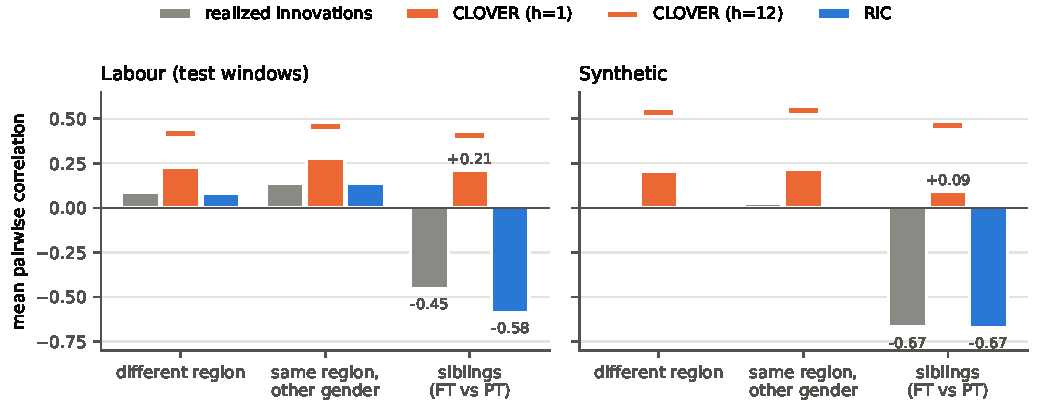
\includegraphics[width=\linewidth]{fig_correlation.pdf}
  \caption{Mean pairwise correlation of bottom series by lowest-common-ancestor class.
  Gray: realized first differences over the 60 months before each test origin and the
  test horizon. Orange: CLOVER's predicted correlation at $h=1$ (bar) and $h=12$
  (tick). Blue: RIC. Labour: three seeds, last-12-months test. Synthetic: three seeds,
  four rolling origins; its sibling relation is built in at a known strength.}
  \label{fig:correlation}
\end{figure}

\section{Method: realized innovation correlation}
\label{sec:method}

RIC keeps every network output that sets a marginal and replaces only the dependence.

\paragraph{Marginals.} From CLOVER's head, the marginal variance of series $i$ at
horizon $\eta$ is $s^2_{i\eta}=\sigma^2_{i\eta}+\lVert\Fmat_{i\eta}\rVert^2$. RIC keeps
$s_{i\eta}$ exactly.

\paragraph{Innovations.} From the window's (normalised) history $y\in\Real^{L\times\Nb}$,
form first differences $x_t = y_t - y_{t-1}$, demean them, and compute their
correlation matrix $\Rhat$. Correlation is invariant to the per-series affine window
scaling, so normalised and raw histories give the same $\Rhat$. Differencing removes
the integrated level that makes co-trending series look correlated. Only history
before the forecast origin is used.

\paragraph{Hierarchy-structured shrinkage.} With $L-1=35$ differences and $\Nb=32$ series,
$\Rhat$ is noisy. Classify each pair $(i,j)$ by the depth of its lowest common ancestor,
read from $\Smat$ alone: the aggregate row with the fewest members containing both, at
depth equal to the number of rows strictly containing it. The target $T$ has unit
diagonal and, for every off-diagonal pair, the mean of $\Rhat$ over that pair's class
in this window. The shrunk correlation is
\begin{equation}
  \mathbf{R} = (1-\lambda)\,\Rhat + \lambda\,T,
  \qquad
  \lambda = \min\!\Big(1,\ \frac{\sum_{i\neq j}\widehat{\operatorname{Var}}(\hat r_{ij})}
  {\sum_{i\neq j}(\hat r_{ij}-t_{ij})^2}\Big),
\end{equation}
with the analytic intensity of \citet{schafer2005shrinkage}, recomputed per window. The
target pools estimates across pairs that share a structural role (siblings, cousins,
others) without assuming independence. An identity target, the default of
\citet{ledoit2004well}-style shrinkage, is the ablation.

\paragraph{Back to a factor model.} Take the top-$K$ eigenpairs $(e_k, v_k)$ of $\mathbf{R}$,
form unit loadings $\tilde f_{ik} = v_{ik}\sqrt{\max(e_k,0)}$ (rows rescaled onto the unit
ball if clipping pushed them past it), and set
\begin{equation}
  \Fmat^{\text{RIC}}_{i\eta} = s_{i\eta}\,\tilde f_i,
  \qquad
  \sigma^{\text{RIC}}_{i\eta} = s_{i\eta}\sqrt{1-\lVert\tilde f_i\rVert^2}.
\end{equation}
The result is again $\operatorname{diag}+$ low rank with marginal variance $s^2_{i\eta}$ and
correlation $\mathbf{R}$ (up to the truncation, which moves residual correlation into
the idiosyncratic term). Denormalisation, reparameterised sampling, clip-then-aggregate
coherence and the CRPS objective are untouched. The only gradient path is through
$s_{i\eta}$. The correlation is computed from data with no learned parameters.

\paragraph{Optional attenuation.} A forecast error contains the network's own mean
error as well as the innovations, and that error is largely idiosyncratic. Forecast
errors are therefore less correlated than innovations: on Labour, $0.033$ against $0.079$
across regions and $-0.38$ against $-0.59$ for siblings. Scaling the unit loadings by
$\sqrt\rho$ maps $\mathbf{R}$ to $\rho\mathbf{R}+(1-\rho)I$ exactly. We report
$\rho=0.8$ as a fixed constant. A learned per-horizon $\rho_\eta$, even reparameterised
to move 20 times faster under Adam, stays near its initial value, because the CRPS
carries too little signal about correlation.

\paragraph{Cost.} One $\Nb\times\Nb$ correlation and one symmetric eigendecomposition per
window, at most $\Nb=200$ here (Traffic). We did not time it separately
\todo{measure wall-clock against CLOVER}.

\section{Experimental setup}
\label{sec:setup}

\paragraph{Datasets.} The five public single hierarchies of the CLOVER benchmark used
throughout this project: Labour, Prison, Tourism-small, Wiki2, Traffic. Each has its
CLOVER configuration unchanged. The \emph{synthetic} hierarchy mirrors Labour's shape
(Total, 4 regions, 8 region--gender groups, 16 bottom series; 480 months). Each group
total is a log random walk with drift, driven by a national shock whose loading fades
from 1 to $0.2$. It splits into full-time and part-time through a share whose logit is
an AR(1) with $\phi=0.97$. Realized sibling innovation correlation runs from $-0.42$ to
$-0.65$ and other pairs from $0.16$ to $0.03$. The model and training settings copy
Labour's, so the synthetic isolates the dependence mechanism under the architecture
CLOVER actually uses there.

\paragraph{Protocols.} The paper's single last-horizon test, plus rolling-origin tests
where a series is long enough: Labour, four non-overlapping 12-month origins; Traffic,
seven daily origins; Synthetic, four 12-month origins. Prison and Tourism-small are
too short for rolling tests.

\paragraph{Seeds and testing.} Seeds 0--11 for every configuration, the same seeds for
CLOVER and RIC (paired), 4 workers $\times$ 2 torch threads. The thread count is fixed
because CLOVER results change with it. Our CLOVER runs reproduce the project's stored
baseline file exactly, seed for seed. Each comparison uses a two-sided Wilcoxon
signed-rank test \citep{wilcoxon1945individual} on the 12 paired overall sCRPS values,
with Holm correction \citep{holm1979simple} across all 16 comparisons in
Table~\ref{tab:main}.

\section{Results}
\label{sec:results}

\begin{table}[t]
  \centering
  \small
  \begin{tabular}{llrrrrrrr}
\toprule
 & & & \multicolumn{3}{c}{RIC} & \multicolumn{3}{c}{RIC, $\rho{=}0.8$} \\
\cmidrule(lr){4-6} \cmidrule(lr){7-9}
Dataset & Test protocol & CLOVER & $\Delta$ & wins & $p_\text{Holm}$ & $\Delta$ & wins & $p_\text{Holm}$ \\
\midrule
Labour & last 12 months & 0.0077 & -2.5\% & 11/12 & 0.274 & -2.7\% & 11/12 & 0.315 \\
Labour & 4 rolling origins & 0.0094 & -0.3\% & 8/12 & 1.000 & -0.4\% & 9/12 & 1.000 \\
Labour, no features & last 12 months & 0.0081 & -3.6\% & 9/12 & 0.274 & -4.2\% & 9/12 & 0.167 \\
Labour, no features & 4 rolling origins & 0.0095 & -1.7\% & 10/12 & 0.068 & \textbf{-2.0\%} & 12/12 & 0.012 \\
Prison & last 8 quarters & 0.0467 & \textbf{-8.6\%} & 12/12 & 0.012 & \textbf{-8.6\%} & 12/12 & 0.012 \\
Tourism-S & last 4 quarters & 0.0682 & +2.9\% & 3/12 & 1.000 & +2.1\% & 5/12 & 1.000 \\
Tourism-L & last 12 months & 0.1286 & -0.4\% & 9/12 & 1.000 & -0.7\% & 8/12 & 1.000 \\
Tourism-L & 4 rolling origins & 0.1395 & -0.2\% & 6/12 & 1.000 & -0.1\% & 6/12 & 1.000 \\
Wiki2 & last 7 days & 0.2480 & +0.2\% & 5/12 & 1.000 & -0.7\% & 8/12 & 1.000 \\
Traffic & last day & 0.0207 & +6.9\% & 4/12 & 1.000 & +4.9\% & 6/12 & 1.000 \\
Traffic & 7 rolling days & 0.0252 & +0.5\% & 7/12 & 1.000 & -2.7\% & 8/12 & 1.000 \\
Synthetic & 4 rolling origins & 0.0056 & \textbf{-4.8\%} & 11/12 & 0.021 & -4.4\% & 9/12 & 0.130 \\
\bottomrule
\end{tabular}

  \caption{Overall sCRPS of CLOVER and relative change $\Delta$ (mean over 12 paired
  seeds) for RIC (tree target, analytic shrinkage) and RIC with attenuation
  $\rho=0.8$. ``wins'' counts seeds on which the variant is better. $p_\text{Holm}$:
  Wilcoxon signed-rank, Holm-adjusted over the 16 comparisons; bold where
  $p_\text{Holm}<0.05$.}
  \label{tab:main}
\end{table}

Table~\ref{tab:main} gives the headline. Holm correction runs over all 20
comparisons. Two results are significant for plain RIC. On Prison it gains $-8.6\%$,
better on all 12 seeds; Prison is a short, integrated hierarchy whose configuration
already carries the paper's features. On the synthetic hierarchy, built to have
Labour's dependence, it gains $-4.8\%$ (11/12). On Labour the result depends on the
baseline. Against the paper-configuration CLOVER (with features), RIC gains $-2.5\%$ on
the paper's test window, better on 11 of 12 seeds (unadjusted $p=0.016$, not
significant after correction), and $-0.3\%$ under rolling origins, which is not
significant. Against the featureless configuration, the gains are larger: $-3.6\%$ and
$-1.7\%$, and with attenuation $-2.0\%$ on all 12 seeds, significant after correction.
The features improve CLOVER's mean forecasts. They leave its dependence wrong, but
they shrink the share of the loss that dependence controls. On the other
three datasets no change is significant. For attenuated RIC, Traffic's single-day
test suggests a loss ($+4.9\%$ mean, $+0.8\%$ median), but the seven-day rolling test
reverses its sign ($-2.7\%$), so that single-day figure should not be read as a loss.
Plain RIC is neutral on the seven-day test ($+0.5\%$, median $-2.3\%$).

Figure~\ref{fig:correlation} shows the mechanism working. On the synthetic hierarchy RIC
predicts sibling correlation $-0.67$ against a true $-0.67$, and other classes $0.015$
and $0.018$ against $0.016$ and $0.022$. CLOVER predicts $+0.09$ to $+0.46$ for siblings.
On Labour RIC's classes are $+0.08$, $+0.14$, $-0.58$ against realized $+0.09$, $+0.14$,
$-0.45$.

\begin{figure}[t]
  \centering
  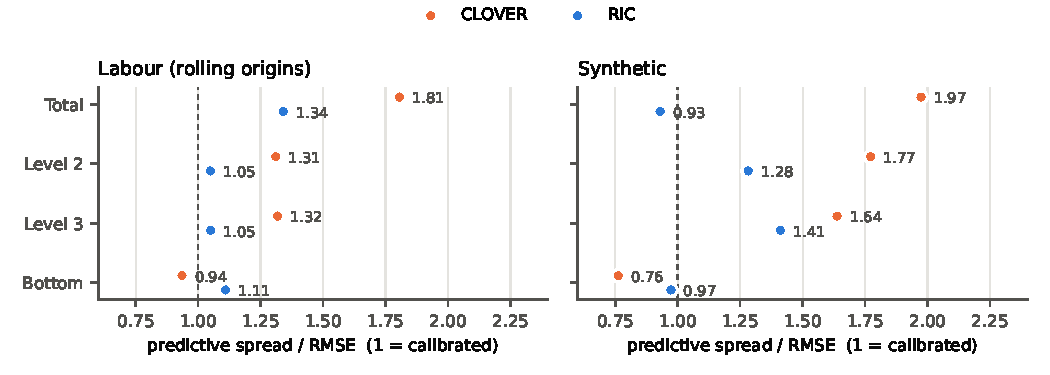
\includegraphics[width=\linewidth]{fig_calibration.pdf}
  \caption{Predictive spread over RMSE by aggregation level, mean over 12 seeds (1 is
  calibrated). CLOVER is too wide at every aggregate and too narrow at the bottom on
  the synthetic data. RIC moves every level toward 1; on Labour the Total stays wide
  (Section~\ref{sec:limitations}).}
  \label{fig:calibration}
\end{figure}

\begin{table}[t]
  \centering
  \small
  \begin{tabular}{lrrrrrrrr}
\toprule
 & \multicolumn{4}{c}{Labour, last 12 months} & \multicolumn{4}{c}{Labour, rolling} \\
\cmidrule(lr){2-5} \cmidrule(lr){6-9}
 & \multicolumn{2}{c}{sCRPS} & \multicolumn{2}{c}{spread/RMSE} & \multicolumn{2}{c}{sCRPS} & \multicolumn{2}{c}{spread/RMSE} \\
Level & CLOVER & RIC & CLOVER & RIC & CLOVER & RIC & CLOVER & RIC \\
\midrule
Total & 0.0036 & 0.0032 & 3.01 & 2.27 & 0.0048 & 0.0046 & 1.63 & 1.21 \\
Geography & 0.0057 & 0.0054 & 1.99 & 1.69 & 0.0080 & 0.0080 & 1.22 & 1.01 \\
Gender $\times$ Geography & 0.0078 & 0.0077 & 1.58 & 1.32 & 0.0091 & 0.0091 & 1.28 & 1.07 \\
Bottom (status) & 0.0135 & 0.0136 & 1.16 & 1.31 & 0.0158 & 0.0157 & 0.92 & 1.07 \\
\bottomrule
\end{tabular}

  \caption{Labour (paper configuration, with features) by aggregation level, mean over
  12 seeds: sCRPS and predictive spread/RMSE for CLOVER and RIC ($\rho=0.8$). The gain
  comes from the aggregates, where dependence decides the spread. The bottom level,
  whose marginals RIC leaves to the network, is unchanged.}
  \label{tab:levels}
\end{table}

Table~\ref{tab:levels} shows where the gain comes from. On the last-12-months test the
Total improves from $0.0036$ to $0.0032$ and Geography from $0.0057$ to $0.0054$, while
the bottom level is unchanged. That is the expected signature of a dependence fix in a
bottom-up coherent model. Under rolling origins RIC brings Geography and
Gender$\times$Geography to calibration ($1.01$, $1.07$ from $1.22$, $1.28$) and the Total
from $1.63$ to $1.21$. Those levels' sCRPS barely moves there, because their loss is
dominated by mean error (Section~\ref{sec:limitations}).

\subsection{Scoring the joint distribution}
\label{sec:joint}

sCRPS scores each series' marginal separately; it sees cross-series dependence only
through the aggregates, where the mean error can mask it. Table~\ref{tab:joint} scores
the joint bottom-level distribution at every forecast step directly. It uses the
energy score \citep{gneiting2007strictly} and the variogram score of order $1/2$
\citep{scheuerer2015variogram}, each bottom series divided by its mean absolute value
over the training rows. The runs are the same 12 seeds; rerunning them for these
scores reproduced every stored sCRPS exactly.

\begin{table}[t]
  \centering
  \small
  \begin{tabular}{llrrrrrrrr}
\toprule
 & & \multicolumn{4}{c}{Energy score} & \multicolumn{4}{c}{Variogram score} \\
\cmidrule(lr){3-6} \cmidrule(lr){7-10}
 & & \multicolumn{2}{c}{RIC} & \multicolumn{2}{c}{$\rho{=}0.8$} & \multicolumn{2}{c}{RIC} & \multicolumn{2}{c}{$\rho{=}0.8$} \\
Dataset & Test protocol & $\Delta$ & wins & $\Delta$ & wins & $\Delta$ & wins & $\Delta$ & wins \\
\midrule
Labour & last 12 months & -0.9\% & 8/12 & -1.0\% & 8/12 & +0.9\% & 4/12 & +0.9\% & 4/12 \\
Labour & 4 rolling origins & -1.1\% & 11/12 & -1.1\% & 11/12 & -0.8\% & 8/12 & -0.8\% & 8/12 \\
Prison & last 8 quarters & \textbf{-5.2\%} & 12/12 & \textbf{-5.4\%} & 12/12 & -2.3\% & 8/12 & -2.4\% & 9/12 \\
Tourism-S & last 4 quarters & +0.0\% & 4/12 & -0.5\% & 6/12 & +0.2\% & 6/12 & -0.1\% & 6/12 \\
Wiki2 & last 7 days & +3.6\% & 1/12 & -1.1\% & 7/12 & +3.4\% & 2/12 & -0.7\% & 7/12 \\
Traffic & 7 rolling days & \textbf{+9.7\%} & 0/12 & \textbf{+5.6\%} & 1/12 & \textbf{+9.1\%} & 0/12 & \textbf{+6.2\%} & 0/12 \\
Synthetic & 4 rolling origins & \textbf{-3.7\%} & 12/12 & \textbf{-3.4\%} & 12/12 & \textbf{-4.8\%} & 12/12 & \textbf{-4.5\%} & 12/12 \\
\bottomrule
\end{tabular}

  \caption{Relative change in the energy and variogram scores of the joint bottom-level
  forecast distribution against CLOVER (paper configuration), mean over 12 paired
  seeds. Bold: Wilcoxon $p<0.05$ after Holm correction over the 28 comparisons in this
  table. Lower is better, so a bold positive entry is a significant loss.}
  \label{tab:joint}
\end{table}

The synthetic hierarchy improves on every seed under both scores. That is the cleanest
evidence that RIC's dependence is better where the truth is known. Prison's energy score
improves on every seed ($-5.2\%$). On Labour the energy score improves on 11 of 12 seeds
under rolling origins ($-1.1\%$, unadjusted $p=0.007$), where sCRPS saw nothing. That
does not survive correction over 28 tests. The variogram score, which also penalises
errors in the differences between series' means, does not move on Labour, whose loss
is dominated by mean error.

Traffic is the counter-example. RIC worsens both joint scores on every seed ($+9.7\%$
and $+9.1\%$; $+5.6\%$ and $+6.2\%$ with attenuation), although its sCRPS was neutral.
Traffic is daily occupancy with weekly seasonality, not an integrated hierarchy, and 55
first differences estimate a $200\times200$ correlation poorly. CLOVER's network, with
its cross-series mixer, learns a better dependence there. Wiki2 is similar but weaker:
plain RIC worsens both scores by about $3.5\%$, while the attenuated version is
neutral. These are costs that the sCRPS-only view in Table~\ref{tab:main} hid.

\section{Ablations}
\label{sec:ablations}

\begin{table}[t]
  \centering
  \small
  \begin{tabular}{lrrrrrr}
\toprule
 & \multicolumn{2}{c}{Labour, last 12 m} & \multicolumn{2}{c}{Labour, rolling} & \multicolumn{2}{c}{Synthetic} \\
\cmidrule(lr){2-3} \cmidrule(lr){4-5} \cmidrule(lr){6-7}
Variant & $\Delta$ & $n$ & $\Delta$ & $n$ & $\Delta$ & $n$ \\
\midrule
RIC: differences, tree target, analytic shrinkage & -3.6\% & 12 & -1.7\% & 12 & -4.8\% & 12 \\
\quad identity target instead of tree & -4.1\% & 12 & -1.6\% & 12 & -4.3\% & 12 \\
\quad fixed shrinkage $\lambda{=}0.5$ toward $I$ & -2.9\% & 5 & -2.7\% & 5 & -- &  \\
\quad levels instead of differences & -0.2\% & 5 & +1.4\% & 5 & -- &  \\
\quad levels, identity target, $\lambda{=}0.5$ & -1.2\% & 12 & +0.3\% & 12 & +0.6\% & 12 \\
\quad no cross-series dependence at all & -3.2\% & 5 & +0.1\% & 5 & -3.1\% & 12 \\
\quad gated mix with the network's own loadings & -2.7\% & 5 & -2.1\% & 5 & -- &  \\
\quad $\eta$-step changes for horizon $\eta$ & -3.9\% & 5 & +1.1\% & 5 & -- &  \\
\quad 60-row estimation history & -3.4\% & 5 & -2.4\% & 5 & -- &  \\
\quad 120-row estimation history & -3.7\% & 5 & +0.5\% & 5 & -- &  \\
\quad full history & -2.0\% & 5 & -2.0\% & 5 & -- &  \\
\quad attenuation $\rho{=}0.8$ & -4.2\% & 12 & -2.0\% & 12 & -4.4\% & 12 \\
\quad attenuation $\rho{=}0.65$ & -4.2\% & 12 & -2.1\% & 12 & -3.9\% & 12 \\
\quad attenuation $\rho{=}0.5$ & -3.5\% & 12 & -2.1\% & 12 & -3.7\% & 12 \\
\quad attenuation, learned $\rho_\eta$ & -3.5\% & 12 & -2.0\% & 12 & -4.3\% & 12 \\
\bottomrule
\end{tabular}

  \caption{Relative change in overall sCRPS against CLOVER on the same seeds; $n$ is
  the number of seeds. Indented rows change one thing from the first row. Rows with
  $n=5$ were run before the 12-seed protocol and are indicative only.}
  \label{tab:ablation}
\end{table}

Table~\ref{tab:ablation} isolates the cause.
\begin{itemize}
  \item \textbf{Differences, not levels.} The same estimator applied to z-scored levels
  gives $-1.2\%$/$+0.3\%$ on Labour and $+0.6\%$ on the synthetic data, none
  significant. That is spurious level correlation reproduced, and it is the central
  control of this report.
  \item \textbf{Dependence matters.} Removing all cross-series dependence helps on one
  Labour protocol and not the other ($-3.2\%$ / $+0.1\%$). It is worse than RIC on the
  synthetic data ($-3.1\%$ against $-4.8\%$), where the true negative sibling
  correlation has to be represented.
  \item \textbf{Target.} Tree and identity targets are within noise on Labour. The
  tree target is better on the synthetic data, where its class structure matches the
  truth.
  \item \textbf{Window, not history.} Estimating from longer histories (60, 120 or all
  rows) does not help consistently, and the full history is worse. Dependence drifts,
  so the most recent window is the right estimate.
  \item \textbf{Horizon-specific correlation} from $\eta$-step changes is unstable
  ($-3.9\%$ and $+1.1\%$ across the two Labour protocols).
  \item \textbf{Attenuation} is flat over $\rho\in[0.5,0.8]$ on Labour and costs a little
  on the synthetic data, where RIC was already calibrated.
\end{itemize}

\subsection{Choosing when to apply RIC, without the test set}
\label{sec:gate}

Since RIC helps integrated hierarchies and hurts Traffic, a practitioner needs a rule
for when to use it. We use a pre-test backtest. It drops the final horizon (the real
test) and scores rolling pseudo-test origins inside the remaining data: 4 for Labour
and Wiki2, 7 for Traffic, 2 for Tourism-S, and 1 for Prison, the most its 40 rows
allow. It runs 5 seeds of CLOVER, RIC and RIC with $\rho=0.8$, and picks whichever
has the lowest backtest score. Table~\ref{tab:gate} compares selecting on sCRPS with
selecting on the energy score.

\begin{table}[t]
  \centering
  \small
  \begin{tabular}{llllll}
\toprule
 & \multicolumn{2}{c}{sCRPS-selected} & \multicolumn{3}{c}{energy-selected} \\
\cmidrule(lr){2-3} \cmidrule(lr){4-6}
Dataset & pick & test energy & pick & test sCRPS & test energy \\
\midrule
Labour & CLOVER & +0.0\% (0/12) & RIC & -0.3\% (8/12) & -1.1\% (11/12) \\
Prison & RIC & -5.2\% (12/12) & RIC & -8.6\% (12/12) & -5.2\% (12/12) \\
Tourism-S & CLOVER & +0.0\% (0/12) & RIC $\rho{=}0.8$ & +2.1\% (5/12) & -0.5\% (6/12) \\
Wiki2 & CLOVER & +0.0\% (0/12) & CLOVER & +0.0\% (0/12) & +0.0\% (0/12) \\
Traffic & RIC $\rho{=}0.8$ & +5.6\% (1/12) & CLOVER & +0.0\% (0/12) & +0.0\% (0/12) \\
\bottomrule
\end{tabular}

  \caption{Backtest-gated selection. ``pick'' is the configuration with the lowest mean
  backtest score; its real-test change against CLOVER is the mean over 12 paired
  seeds (wins in parentheses). Labour is scored on four rolling origins (paper
  configuration), Traffic on seven rolling days.}
  \label{tab:gate}
\end{table}

Selecting on sCRPS fails in both directions. It rejects RIC on Labour. It accepts RIC
on Traffic, at a $+5.6\%$ energy-score loss. On Prison it was a coin-flip (backtest
margin $0.07\%$). Selecting on the energy score makes the call that the 12-seed test
results support on every dataset. It keeps RIC on Labour and Prison (backtest
$-1.0\%$ and $-6.6\%$) and rejects it on Wiki2 and Traffic. On Tourism-S it picks
attenuated RIC on a $-0.7\%$ margin; the test results there are neutral in every
score. Even from a single pseudo-origin, the joint score separates Prison clearly
where sCRPS could not. The energy-gated procedure leaves no dataset significantly
worse on any score. It averages $-1.4\%$ in both sCRPS and energy score over the five
datasets, and $-8.6\%$ / $-5.2\%$ on Prison. This is the deployable form of the
method: RIC behind a joint-score backtest gate.

\section{What did not work}
\label{sec:negative}

Mean-side error correction (Johansen or share-based vectors, an error-correction skip,
trend-constrained loadings) tied CLOVER everywhere. This is now explained: the mean was
not where the loss was. Learned shrinkage and learned attenuation stayed at their
initial values within CLOVER's step budget, the same Adam step-budget limitation the
earlier error-correction skip hit. On Tourism-small, whose 8-row window leaves seven
first differences for 56 series, neither seasonal differencing ($y_t-y_{t-4}$) nor the
full pre-origin history helped: $+5.1\%$ with both combined, 5 seeds. That hierarchy
is quarterly and short (36 rows), and its dependence is not estimable this way.

\paragraph{The remaining mean error is not cheaply forecastable.} On Labour (paper
configuration, RIC, three seeds) about $60\%$ of the bottom level's per-origin bias is
a mis-split within full-time/part-time pairs, not an error in the pair's sum. Keeping
each pair's predicted sum and re-splitting it by the last observed share, or by the
window-average share, leaves every aggregate unchanged by construction. It makes the
bottom level worse by $5$--$7\%$ on both protocols. The network's own split already
beats a random-walk or mean-reverting share forecast, so the within-pair bias left on
the table looks like unforecastable share shocks, not a missed error-correction
signal. This agrees with the earlier mean-side ties.

\section{Limitations and threats to validity}
\label{sec:limitations}

\begin{itemize}
  \item \textbf{Baseline level.} With the paper's features our CLOVER scores $0.0077$ on
  Labour; the paper reports $0.0074$, and PERMBU-MinT $0.0067$. The remaining $0.0003$
  may come from the lookback (36 months here; the paper does not state it) or from
  the estimator. The claim is therefore relative to our CLOVER, not a row in the
  paper's table. \todo{check input size and sCRPS estimator against the paper's code}
  \item \textbf{Labour's gain depends on the baseline.} Most of RIC's Labour gain over
  the featureless configuration disappears once the paper's features are added. The
  dependence error remains, but the features remove much of the loss it accounted
  for. The robust Labour claim is the corrected dependence and calibration, not a
  large score change.
  \item \textbf{Remaining Labour gap.} The Total stays wide (spread/RMSE $1.28$ rolling,
  $1.95$ on the single window), and no attenuation removes it without losing elsewhere.
  Below the Total, about $55\%$ of squared error is per-origin bias in the mean, which
  no dependence model can address. Simple share-based re-anchoring does not recover it
  (Section~\ref{sec:negative}).
  \item \textbf{Short series.} Prison and Tourism-small give RIC 7 differences per window.
  Prison still gains strongly, but neither supports rolling tests or a reliable
  backtest gate.
  \item \textbf{Single-window tests.} The paper's protocol scores one horizon per
  dataset. Traffic shows that this alone can flip a sign, which is why rolling origins
  are reported wherever the data allows.
  \item \textbf{Scope.} RIC helps where series are integrated and related through the
  hierarchy (Labour, Prison, the synthetic data). On Traffic it significantly worsens
  the joint distribution (Section~\ref{sec:joint}), and on Wiki2 plain RIC does too, so
  it must not be applied blindly. A backtest gate on the energy score handles this on
  all five datasets (Section~\ref{sec:gate}). A gate on sCRPS does not, and neither
  does a unit-root test: ADF flags $85\%$ of Traffic's series, about the same share as
  Prison's. The gate is validated on five datasets only, and with 5 backtest seeds.
\end{itemize}

\section{Reproduction}
\label{sec:repro}

From the repository root (no core module is modified; everything lives in
\texttt{experiments/ric\_clover/}):
\begin{verbatim}
python experiments/ric_clover/bench.py --datasets labour --origins 4 \
    --variants base ric_tree ric_tree_att1 --seeds 0 1 2 3 4 5 6 7 8 9 10 11 \
    --out experiments/ric_clover/results/labour_roll4.jsonl
python experiments/ric_clover/stats.py experiments/ric_clover/results/labour_roll4.jsonl \
    --variants ric_tree ric_tree_att1
python experiments/ric_clover/diag_corr.py --dataset labour --variants base ric_tree
python experiments/ric_clover/build_synthetic_ric.py
python experiments/ric_clover/bench.py --backtest 4 --datasets labour ...
python experiments/ric_clover/make_report_assets.py   # tables/ and figures here
\end{verbatim}
\texttt{configs/datasets/labour.yaml} now carries the paper's static and calendar
features, so the commands above run the paper configuration. To reproduce the
featureless Labour rows, add
\verb|--set "features.static=[]" --set "features.future=[]"|.
Calibration-by-era and oracle-debiasing numbers in Section~\ref{sec:diagnosis} come from
one-off diagnostics run during the investigation and are not yet scripted
\todo{script them before submission}.

\section{Conclusion}

CLOVER's weakness on cointegrated hierarchies is a dependence failure, not a mean
failure. A per-series head reading z-scored levels predicts the uniform positive
correlation that co-trending levels suggest, while the innovations that decide the
spread of aggregates carry negative within-parent correlation and a fading common
component. Re-estimating dependence in every window from differences, with
hierarchy-structured shrinkage, keeps CLOVER's coherence-by-construction intact. It
fixes the dependence where the truth is known. It improves Prison significantly and
Labour's paper test window on 11 of 12 seeds, and corrects Labour's aggregate
calibration. On a daily seasonal hierarchy whose learned dependence is already good
(Traffic) it is harmful in the joint scores. A pre-test backtest that selects on the
energy score separates the two cases on all five datasets, which makes RIC safe to
deploy. What remains of Labour's gap is in the mean.

\bibliographystyle{plainnat}
\bibliography{../paper/references,references_ric}

\end{document}
